\documentclass{beamer}
\usepackage[utf8]{inputenc}
\usepackage{pgfplots}
\usepackage{tikz}
\usepackage{float}
\usetikzlibrary{positioning,shapes,shadows,arrows,chains}
\usepackage{mathtools,amsfonts,amssymb}
\usepackage{graphicx}
\usepackage{minted}
\usetheme{Singapore}
\setbeamertemplate{footline}[frame number]

\tikzset{
	cell/.style={
		rectangle split,
		rectangle split parts=4,
		rectangle split horizontal,
		rectangle split part fill={lightgray!30},
		rectangle split empty part width=0.1cm,
		draw
	}
}

\begin{document}

\title{Alignment in C}
\subtitle{Seminar "Effiziente Programmierung in C"}
\date{2014-01-09}
\author{Sven-Hendrik Haase}
\institute{Universität Hamburg, Fakultät für Informatik}

\begin{frame}
    \titlepage
\end{frame}
%It's basically like Tetris but with computer memory

\begin{frame}{Outline}
    \tableofcontents
\end{frame}

\section{Introduction}
\subsection{Memory addressing}
\begin{frame}{\insertsection}{\insertsubsection}
	\begin{itemize}
		\item Computers address memory in word sized chunks
		\item A \textbf{word} is a computer's natural unit for data
		\item Word size is defined by architecture
		\item 4 byte on 32-bit, 8 byte on 64-bit
		\item This means we can only address data at memory locations that are
			  multiples of 4 or 8 respectively\pause\
		\item Graphical example for 4 byte words:
	\end{itemize}

	\begin{center}
		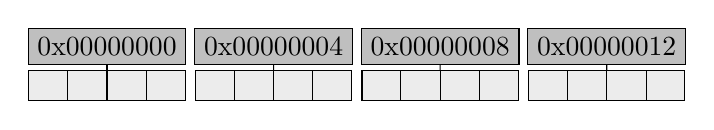
\begin{tikzpicture}[start chain, level distance=0.5cm, node distance=0.1cm, every on chain/.style={draw, fill=lightgray, minimum width=2cm}]
			\node [on chain] {0x00000000} child {node [cell] {}};
			\node [on chain] {0x00000004} child {node [cell] {}};
			\node [on chain] {0x00000008} child {node [cell] {}};
			\node [on chain] {0x00000012} child {node [cell] {}};
		\end{tikzpicture}
	\end{center}
\end{frame}

\subsection{Alignment 101}
\begin{frame}{\insertsection}{\insertsubsection}
	\begin{itemize}
		\item Assume a 32-bit architecture with a word size of 4 byte
		\item Let's save a 4 byte \textbf{int}
			\tikz[baseline=-0.5ex]{ \node[cell, rectangle split part fill={green!50},] {};} in our memory: \pause
	\end{itemize}
	\begin{center}
		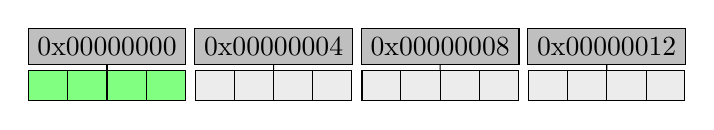
\begin{tikzpicture}[start chain, level distance=0.5cm, node distance=0.1cm, every on chain/.style={draw, fill=lightgray, minimum width=2cm}]
			\node [on chain] {0x00000000} child {node [cell, rectangle split part fill={green!50},] {}};
			\node [on chain] {0x00000004} child {node [cell] {}};
			\node [on chain] {0x00000008} child {node [cell] {}};
			\node [on chain] {0x00000012} child {node [cell] {}};
		\end{tikzpicture}
	\begin{itemize}
		\item Looks good!
	\end{itemize}
	\end{center}
\end{frame}

\begin{frame}{\insertsection}{\insertsubsection}
	\begin{itemize}
		\item Let's save a \textbf{char}
			\tikz[baseline=-0.5ex]{ \node[cell, rectangle split part fill={red!50,lightgray!30}] {};}, a \textbf{short}
			\tikz[baseline=-0.5ex]{ \node[cell, rectangle split part fill={blue!50,blue!50,lightgray!30}] {};} and an \textbf{int}
			\tikz[baseline=-0.5ex]{ \node[cell, rectangle split part fill={green!50},] {};} in our memory: \pause
	\end{itemize}
	\begin{center}
		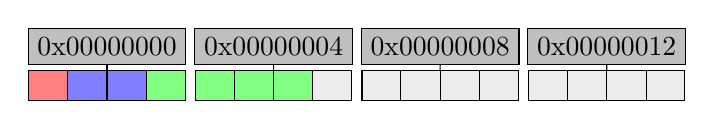
\begin{tikzpicture}[start chain, level distance=0.5cm, node distance=0.1cm, every on chain/.style={draw, fill=lightgray, minimum width=2cm}]
			\node [on chain] {0x00000000} child {node [cell, rectangle split part fill={red!50,blue!50,blue!50,green!50}] {}};
			\node [on chain] {0x00000004} child {node [cell, rectangle split part fill={green!50,green!50,green!50,lightgray!30}] {}};
			\node [on chain] {0x00000008} child {node [cell] {}};
			\node [on chain] {0x00000012} child {node [cell] {}};
		\end{tikzpicture}
	\begin{itemize}
		\item Oh wait \pause
		\item Needs two memory accesses and some logic to fetch the \textbf{int}.
	\end{itemize}
	\end{center}
\end{frame}

\begin{frame}{\insertsection}{\insertsubsection}
	\begin{itemize}
		\item We need to be smarter about this!
		\item Padding \tikz[baseline=-0.5ex]{ \node[cell, rectangle split part fill={darkgray,lightgray!30},] {};} to the rescue\pause
	\end{itemize}
	\begin{center}
		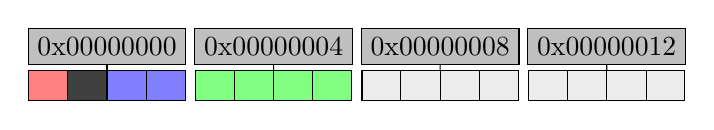
\begin{tikzpicture}[start chain, level distance=0.5cm, node distance=0.1cm, every on chain/.style={draw, fill=lightgray, minimum width=2cm}]
			\node [on chain] {0x00000000} child {node [cell, rectangle split part fill={red!50,darkgray,blue!50,blue!50}] {}};
			\node [on chain] {0x00000004} child {node [cell, rectangle split part fill={green!50}] {}};
			\node [on chain] {0x00000008} child {node [cell] {}};
			\node [on chain] {0x00000012} child {node [cell] {}};
		\end{tikzpicture}
	\begin{itemize}
		\item Much better
		\item This is considered \textbf{naturally aligned}
	\end{itemize}
	\end{center}
\end{frame}

\subsection{Consquences of misalignment}
\begin{frame}{\insertsection}{\insertsubsection}
	\begin{itemize}
		\item Different behavior depending on architecture
		\item Alignment faul errors on some platforms
		\item Bad performance on others
		\item SSE requires proper alignment
	\end{itemize}
\end{frame}

\section{Data Structure Alignment}
\subsection{Structs and stuff}
\begin{frame}[fragile]{\insertsection}{\insertsubsection}
\begin{minted}{c}
    struct Foo {
        char x; // 1 byte
        int y; // 4 byte
    };
\end{minted}
\end{frame}

\subsection{Performance implications}
\begin{frame}{\insertsection}{\insertsubsection}
	code and shit
\end{frame}

\subsection{SSE}
\begin{frame}{\insertsection}{\insertsubsection}
	code and stuff
\end{frame}

\section{Stack Alignment}
\subsection{Introduction}
\begin{frame}{\insertsection}{\insertsubsection}
	Even More Stuff
\end{frame}

\subsection{Stack Realignment}
\begin{frame}{\insertsection}{\insertsubsection}
	Even More Stuff
\end{frame}

\section{Summary}
\begin{frame}{\insertsection}{\insertsubsection}
	Summary stuff
\end{frame}

\begin{frame}{Resources}
	stuff
\end{frame}

\end{document}
